% !TeX root = er.tex

\chapter{Mapeamento}\label{ch.mapping}

Vimos que um robô pode usar sua capacidade de detectar obstáculos para se localizar, com base em informações sobre a posição dos obstáculos ou outras informações sobre o meio ambiente. Estas informações são normalmente fornecidas por um mapa. É relativamente fácil construir um mapa de ambientes industriais, como fábricas, já que as máquinas estão ancoradas em locais fixos. Os mapas são menos relevantes para um aspirador robótico, pois o fabricante não pode preparar mapas dos apartamentos de cada cliente. Além disso, os robôs seriam muito difíceis de usar se os clientes tivessem que construir mapas de seus apartamentos e mudá-los sempre que um móvel é movimentado. Escusado será dizer que é impossível construir com antecedência mapas de locais inacessíveis como o fundo do mar.

A solução é que o robô construa seu próprio mapa do ambiente. Para construir um mapa é necessária a localização para que o robô saiba onde ele está, mas a localização precisa de um mapa, que precisa \ldots. Para superar este problema de galinha e ovo, os robôs utilizam algoritmos de \emph{localização e mapeamento simultâneos (SLAM)}. Para realizar o SLAM, os robôs utilizam informações conhecidas como válidas mesmo em partes inexploradas do ambiente, refinando as informações durante a exploração.

Isto é o que os humanos fizeram para criar mapas geográficos. Observações do sol e das estrelas foram usadas para localização e os mapas foram criados à medida que a exploração prosseguia. Inicialmente, as ferramentas de localização eram pobres: é relativamente fácil medir a latitude usando um sextante para observar a altura do sol ao meio-dia, mas medidas precisas de longitude eram impossíveis até que relógios precisos chamados cronômetros foram desenvolvidos no final do século XVIII. À medida que a localização melhorou, também melhoraram os mapas, incluindo não apenas a terra e as costas do mar, mas também características do terreno como lagos, florestas e montanhas, bem como estruturas artificiais como edifícios e estradas.

As seções~\ref{s.maps}--\ref{s.grids} introduzem métodos de representação de mapas em um computador. A seção~\ref{s.map-create} descreve como um robô pode criar um mapa usando o algoritmo de fronteira. A seção~\ref{s.map-update} explica como o conhecimento parcial do ambiente ajuda na construção de um mapa. Um algoritmo SLAM é o assunto das três últimas seções.  O algoritmo é apresentado pela primeira vez na seção Sect.~\ref{s.slam-numerical} usando um exemplo relativamente simples. As atividades para SLAM são coletadas na seção Sect.~\ref{s.slam-activities} e a seção Sect.~\ref{s.slam-formal} explica o algoritmo formal.


\section{Mapas discretos e contínuos}\label{s.maps}

Estamos acostumados a mapas gráficos que são impressos em papel, ou, mais comumente hoje em dia, exibidos em computadores e smartphones. Um robô, entretanto, precisa de uma representação não visual de um mapa que possa armazenar em sua memória. Existem duas técnicas para armazenar mapas: mapas discretos (também chamados \emph{grid maps}) e mapas contínuos.

A figura~\ref{fig.disc} mostra um mapa de $8\times 8$ com um objeto triangular. A localização do objeto é armazenada como uma lista das coordenadas de cada célula de grade coberta pelo objeto. O objeto na figura é composto pelas células em:
\[
(5,3),\, (5,4),\, (5,5)\,, (4,5)\,, (5,6),\, (4,6),\, (3,6)\,.
\]
\begin{figure}
\begin{minipage}{.45\textwidth}
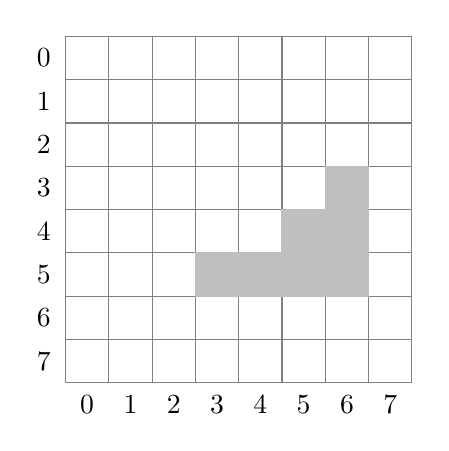
\begin{tikzpicture}[scale=1.1]
\draw[step=5mm,gray] (0,0) grid (4,4);
\foreach \r in {0,1,2,3,4,5,6,7}
  \node at (-.25,3.75-\r*.5) {$\r$};
\foreach \c in {0,1,2,3,4,5,6,7}
  \node at (.25+\c*.5,-.25) {$\c$};
\foreach \x/\y in {3/2, 4/2, 5/2, 6/2, 5/3, 6/3, 6/4}
   \draw[fill,gray!50] (\x/2,\y/2) rectangle +(5mm,5mm);
\path (4.1,0) -- (4.1,4.1); % Avoid truncation
\end{tikzpicture}
\caption{Um mapa discreto das células ocupadas de um objeto}\label{fig.disc}
\end{minipage}
\hspace{\fill}
\begin{minipage}{.45\textwidth}
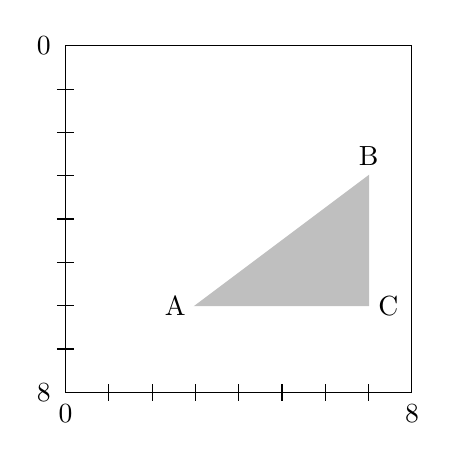
\begin{tikzpicture}[scale=1.1]
\draw (0,0) rectangle +(4,4);
\node at (-.25,0) {$8$};
\node at (-.25,4) {$0$};
\node at (0,-.25) {$0$};
\node at (4,-.25) {$8$};
\foreach \x in {1,2,3,4,5,6,7}
  \draw (\x*.5,-.1) -- (\x*.5,.1);
\foreach \y in {1,2,3,4,5,6,7}
  \draw (-.1,\y*.5) -- (.1,\y*.5);
\draw[fill,gray!50] (3/2,2/2) node[black,left] {\p{A}} -- (7/2,2/2) node[black,right] {\p{C}} -- (7/2,5/2) node[black,above] {\p{B}} -- cycle;
\path (4.1,0) -- (4.1,4.1); % Avoid truncation
\end{tikzpicture}
\caption{Um mapa contínuo do mesmo objeto}
\label{fig.cont}
\end{minipage}
\end{figure}

%\begin{figure}
%\subfigures
%\begin{minipage}{\textwidth}
%\leftfigure[c]{
%\begin{tikzpicture}[scale=1.2]
%\draw[step=5mm,gray] (0,0) grid (4,4);
%\foreach \r in {0,1,2,3,4,5,6,7}
%  \node at (-.25,3.75-\r*.5) {$\r$};
%\foreach \c in {0,1,2,3,4,5,6,7}
%  \node at (.25+\c*.5,-.25) {$\c$};
%\foreach \x/\y in {3/2, 4/2, 5/2, 6/2, 5/3, 6/3, 6/4}
%   \draw[fill,gray!50] (\x/2,\y/2) rectangle +(5mm,5mm);
%\path (4.1,0) -- (4.1,4.1); % Avoid truncation
%\end{tikzpicture}
%}
%\hspace{\fill}
%\rightfigure[c]{
%\begin{tikzpicture}[scale=1.2]
%\draw (0,0) rectangle +(4,4);
%\node at (-.25,0) {$8$};
%\node at (-.25,4) {$0$};
%\node at (0,-.25) {$0$};
%\node at (4,-.25) {$8$};
%\foreach \x in {1,2,3,4,5,6,7}
%  \draw (\x*.5,-.1) -- (\x*.5,.1);
%\foreach \y in {1,2,3,4,5,6,7}
%  \draw (-.1,\y*.5) -- (.1,\y*.5);
%\draw[fill,gray!50] (3/2,2/2) node[black,left] {\p{A}} -- (7/2,2/2) node[black,right] {\p{C}} -- (7/2,5/2) node[black,above] {\p{B}} -- cycle;
%\path (4.1,0) -- (4.1,4.1); % Avoid truncation
%\end{tikzpicture}
%}
%\leftcaption{A discrete map of the occupied cells of an object}\label{fig.disc}
%\rightcaption{A continuous map of the same object\label{fig.cont}}
%\end{minipage}
%\end{figure}

A figura~\ref{fig.cont} mostra um \emph{mapa contínuo} do mesmo objeto. Em vez de armazenar as posições do objeto, as coordenadas das posições de limite são armazenadas:
\[
A = (6,3),\, B = (3,7),\, C = (6,7)\,.
\]
Os mapas discretos não são muito precisos: é difícil reconhecer o objeto na Fig.~\ref{fig.disc} como um triângulo. Para melhorar a precisão, uma grade mais fina deve ser usada: $16\times 16$ ou até $256\times 256$. Naturalmente, à medida que o número de pontos da grade aumenta, o tamanho da memória no robô também deve aumentar. Além disso, um computador mais potente deve ser usado para processar as células da grade. Os robôs móveis têm restrições de peso, custo, capacidade da bateria, e assim por diante, portanto, grades muito finas podem não ser práticas. 

Se os objetos no ambiente são poucos e têm uma forma simples, um mapa contínuo é mais eficiente, além de ser mais preciso. Na Fig.~\ref{fig.cont}, três pares de números representam o triângulo com muito mais precisão do que os sete pares do mapa discreto. Além disso, é fácil de calcular se um ponto está no objeto ou não está usando geometria analítica. Entretanto, se houver muitos objetos ou se eles tiverem formas muito complexas, os mapas contínuos não são mais eficientes nem na memória nem na quantidade de computação necessária. O objeto na Fig.~\ref{fig.cont} é limitado por linhas retas, mas se o limite fosse descrito por curvas de alta ordem, o cálculo se tornaria difícil. Considere um mapa com objetos de $32$ do tamanho um, nenhum deles tocando um no outro. O mapa discreto teria coordenadas de $32$, enquanto o mapa contínuo precisaria armazenar as coordenadas dos quatro cantos de cada objeto.

Na robótica móvel, mapas discretos são comumente usados para representar mapas de ambientes, como fizemos no Chap.~\ref{ch.local}.

\section{O conteúdo das células de um mapa em grade}\label{s.grids}

Um mapa geográfico utiliza notações convencionais para descrever o ambiente. As cores são usadas: verde para florestas, azul para lagos, vermelho para rodovias. São usados símbolos: pontos de vários tamanhos para denotar vilarejos e cidades, e linhas para estradas, onde a espessura e a cor de uma linha é usada para indicar a qualidade da estrada. Os robôs usam mapas de grade onde cada célula armazena um número e nós precisamos decidir o que um número codifica.

A codificação mais simples é a de alocar um bit para cada célula. Um valor de $1$ indica que um objeto existe naquela célula e um valor de $0$ indica que a célula está vazia. Na Fig.~\ref{fig.disc}, cinza representa o valor $1$ e branco representa o valor $0$.

Entretanto, os sensores não são precisos e pode ser difícil ter certeza se uma célula está ou não ocupada por um objeto. Portanto, faz sentido atribuir uma probabilidade a cada célula indicando o quão certo estamos de que o objeto está naquela célula. Figura~\ref{fig.prob-grid} é uma cópia da Fig.~\ref{fig.disc} com as probabilidades listadas para cada célula. Células sem um número são assumidas como tendo uma probabilidade de $0$.

\begin{figure}
\begin{center}
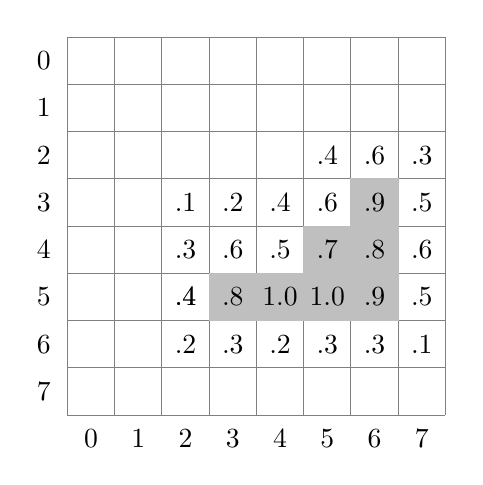
\begin{tikzpicture}[scale=1.2]
\draw[step=5mm,gray] (0,0) grid (4,4);
\foreach \r in {0,1,2,3,4,5,6,7}
  \node at (-.25,3.75-\r*.5) {$\r$};
\foreach \c in {0,1,2,3,4,5,6,7}
  \node at (.25+\c*.5,-.25) {$\c$};
\foreach \x/\y in {3/2, 4/2, 5/2, 6/2, 5/3, 6/3, 6/4}
   \draw[fill,gray!50] (\x/2,\y/2) rectangle +(5mm,5mm);
\foreach \x/\y/\p in {3/2/$.8$, 4/2/$1.0$, 5/2/$1.0$, 6/2/$.9$, 5/3/$.7$, 6/3/$.8$, 6/4/$.9$, 2/2/$.4$, 2/2/$.4$, 2/3/$.3$, 3/3/$.6$, 4/3/$.5$, 5/4/$.6$, 3/4/$.2$, 4/4/$.4$, 2/4/$.1$, 5/5/$.4$, 6/5/$.6$, 7/5/$.3$, 7/4/$.5$, 7/3/$.6$, 7/2/$.5$, 7/1/$.1$, 6/1/$.3$, 5/1/$.3$, 4/1/$.2$, 3/1/$.3$, 2/1/$.2$ }
   \node at (\x/2+.25,\y/2+.25) {\p};
\path (4.1,0) -- (4.1,4.1); % Avoid truncation
\end{tikzpicture}
\caption{Um mapa de grade probabilístico}\label{fig.prob-grid}
\end{center}
\end{figure}

Pode-se ver que as células com uma probabilidade de pelo menos $,7$ são as consideradas na Fig.~\ref{fig.disc} como células ocupadas pelo objeto. Naturalmente, somos livres para escolher algum outro limite, por exemplo $,5$, neste caso mais células são consideradas como ocupadas. Neste exemplo, sabemos que o objeto é triangular, então podemos ver que um limiar de $,5$ torna o objeto maior do que ele realmente é, enquanto que o limiar mais alto $,7$ dá uma melhor aproximação.

\begin{framed}
\act{Mapa probabilístico de obstáculos}{obstacle-map}
\begin{itemize}
\item Coloque seu robô em uma linha na frente de um conjunto de obstáculos que o robô pode detectar com um sensor lateral (Fig.~\ref{fig.mapping-activity}). Se você implementou a localização conforme descrito em Activity~\ref{act.local-uncertain}, você pode usar esta informação para estabelecer onde o robô está. Caso contrário, desenhe linhas regulares no chão que possam ser lidas pelo robô para localização. Construa um mapa probabilístico dos obstáculos.
\item Como as probabilidades mudam quando os obstáculos são adicionados ou removidos?
\end{itemize}
\end{framed}

\begin{figure}
\begin{center}
\begin{tikzpicture}
\draw[fill,lightgray] (-1,-2.5mm) rectangle +(8,5mm);
\pic[scale=1.2] at (0,-5mm) { robot2 };
\foreach \x in {-10mm, 5mm, 20mm, 35mm, 50mm, 65mm}
  \draw[fill,lightgray] (\x,-12mm) rectangle +(3mm,6mm);
\draw[fill] (5,1) rectangle +(12mm,5mm);
\draw[fill] (2,1) rectangle +(12mm,5mm);
\draw[dashed,thick] (15mm,4mm) -- +(20:10mm);
\draw[dashed,thick] (12mm,5mm) -- +(100:10mm);
\end{tikzpicture}
\end{center}
\caption{Os retângulos negros são os obstáculos a serem medidos. A linha cinza orienta o robô e as marcas cinzas são usadas para a localização}\label{fig.mapping-activity}
\end{figure}

\section[O algoritmo de fronteira]{Criação de um mapa por exploração: O algoritmo de fronteira}\label{s.map-create}

Considere um aspirador robótico recém-abandonado em seu apartamento. Obviamente, ele não vem pré-programado com um mapa de seu apartamento. Ao invés disso, ele deve explorar o ambiente para reunir informações que serão usadas para construir seu próprio mapa. Há várias maneiras de explorar o ambiente, a mais simples das quais é a exploração aleatória. A exploração será muito mais eficiente se o robô tiver um mapa parcial que possa utilizar para orientar sua exploração.

\subsection{Mapas de grade com probabilidades de ocupação}

O mapa na Fig.~\ref{fig.map-explore} é um mapa em grade onde cada célula é etiquetada com seu \emph{obstáculo de probabilidade}, que é a probabilidade de haver um obstáculo na célula. O obstáculo pode ser uma parede, uma mesa ou qualquer coisa que não permita que o robô passe por esta célula. Os pontos de interrogação representam células que ainda não foram exploradas. Na ausência de qualquer conhecimento sobre o conteúdo de uma célula, podemos assumir que a probabilidade de haver um obstáculo é de US$ 0,5$, uma vez que poderia ser ocupado com a mesma facilidade ou não. Um ponto de interrogação é usado ao invés do valor de $0,5$ para esclarecer o estado inexplorado das células.

\begin{figure}
\begin{center}
\includegraphics[width=\textwidth]{grid-mapping1.pdf}
\end{center}
\caption{Mapa de grade de um ambiente com probabilidades de ocupação}\label{fig.map-explore}
\end{figure}

O centro do mapa está livre de obstáculos e as probabilidades de ocupação destas células, chamadas \emph{células abertas}, são baixas ($0,1$ ou $0,2$). Existem três obstáculos conhecidos, no canto superior direito, no canto superior esquerdo e no centro inferior. Os obstáculos são caracterizados por altas probabilidades de ocupação ($0,9$ ou $1,0$) e são denotados por células cinzentas. Uma \emph{célula de fronteira} é uma célula aberta adjacente (esquerda, direita, para cima, para baixo) a uma ou mais células desconhecidas. O conjunto de células fronteiriças é chamado de \emph{frontier}. As linhas vermelhas de pequenos quadrados em Fig.~\ref{fig.map-explore} representam a fronteira entre a fronteira e as células desconhecidas no ambiente. As células desconhecidas adjacentes à fronteira são as interessantes que devem ser exploradas a fim de expandir o mapa atual.

\subsection{O algoritmo de fronteira}

O algoritmo \emph{frontier} é usado para expandir o mapa, explorando a fronteira. O robô se move para a célula fronteiriça mais próxima, detecta se há obstáculos em células adjacentes desconhecidas e atualiza o mapa de acordo. 

O mapa de grade na Fig.~\ref{fig.map-explore1} é o mesmo que o mapa na Fig.~\ref{fig.map-explore} com a adição do robô que ocupa uma célula colorida de azul. A célula fronteiriça mais próxima do robô é a célula dois passos acima de sua localização inicial. A seta mostra que o robô se moveu para aquela célula. O robô usa seus sensores locais para determinar se existem obstáculos em células adjacentes desconhecidas. (Os sensores podem detectar obstáculos em todas as oito células adjacentes, incluindo as que se encontram na diagonal). Suponha que a célula superior esquerda certamente contenha um obstáculo (probabilidade $1,0$), enquanto as células diretamente acima e à direita quase certamente não contêm um obstáculo (probabilidade $0,1$). A figura~\ref{fig.map-explore2} mostra o mapa atualizado com estas novas informações e a nova posição da fronteira.


\begin{figure}
\begin{center}
\includegraphics[width=\textwidth]{grid-mapping1b.pdf}
\end{center}
\caption{O robô se move para a fronteira}\label{fig.map-explore1}
\end{figure}

\begin{figure}
\begin{center}
\includegraphics[width=\textwidth]{grid-mapping1c.pdf}
\end{center}
\caption{O robô atualiza células desconhecidas adjacentes à fronteira}\label{fig.map-explore2}
\end{figure}

A figura~\ref{fig.map-explore3} mostra o resultado da próxima iteração do algoritmo. O robô subiu uma célula para a célula de fronteira mais próxima, detectou obstáculos nas duas células desconhecidas adjacentes e atualizou o mapa. O obstáculo superior direito é completamente conhecido e não há célula fronteiriça nas proximidades da posição atual do robô.

\begin{figure}
\begin{center}
\includegraphics[width=\textwidth]{grid-mapping1d.pdf}
\end{center}
\caption{Segunda iteração do algoritmo de fronteira}\label{fig.map-explore3}
\end{figure}

A figura~\ref{fig.map-explore4} mostra a próxima iteração do algoritmo. O robô é bloqueado pelo obstáculo superior direito e tem que evitá-lo ao se deslocar para a célula fronteiriça mais próxima.

A Figura~\ref{fig.map-explore5} mostra o mapa completo construído pelo robô depois de ter explorado toda a fronteira, como mostrado pelo caminho com as setas azuis. 

O algoritmo Algoritmo~\ref{alg.frontier} formaliza o algoritmo da fronteira. Para simplificar, o algoritmo recompila a fronteira em cada etapa. Um algoritmo mais sofisticado examinaria as células em uma vizinhança da posição do robô e adicionaria ou removeria as células cujo status como células de fronteira tenha mudado.

O exemplo ao qual aplicamos o algoritmo de fronteira é um ambiente relativamente simples que consiste em duas salas conectadas por uma porta (na sexta coluna da esquerda na Fig.~\ref{fig.map-explore5}), mas de outra forma fechadas ao ambiente externo. Entretanto, o algoritmo de fronteira funciona em ambientes mais complexos. 

\begin{figure}
\begin{center}
\includegraphics[width=\textwidth]{grid-mapping1e.pdf}
\end{center}
\caption{O robô evita um obstáculo ao se deslocar para a próxima fronteira}\label{fig.map-explore4}
\end{figure}

\begin{figure}
\begin{center}
\includegraphics[width=\textwidth]{grid-mapping1f.pdf}
\end{center}
\caption{O mapa construído pelo algoritmo de fronteira e o caminho explorado pelo robô}\label{fig.map-explore5}
\end{figure}

\begin{figure}
\begin{alg}{Algoritmo de fronteira}{frontier}
\hline
&\idv{}float array grid&// Grid map\\
&\idv{}cell list frontier&// List of frontier cells\\
&\idv{}cell robot& // Cell with robot\\
&\idv{}cell closest&// Closest cell to robot\\
&\idv{}cell c&// Index over cells\\
&\idv{}float low&// Low occupancy probability\\
\hline
\stl{}&loop&\\
\stl{}&\idc{}frontier \ass{} empty&\\
\stl{}&\idc{}for all known cells c  in the grid&\\
\stl{}&\idc{}\idc{}if grid(c) $<$ low and&\\
\stl{}&\idc{}\idc{}\idc{}exists unknown neighbor of c&\\
\stl{}&\idc{}\idc{}\idc{}\idc{}append c to frontier&\\
\stl{}&\idc{}exit if frontier empty&\\
&&\\
\stl{}&\idc{}closest \ass{} cell in frontier nearest robot&\\
\stl{}&\idc{}robot \ass{} closest&\\
\stl{}&\idc{}for all unknown neighbors c of closest&\\
\stl{}&\idc{}\idc{}\idc{}sense if c is occupied&\\
\stl{}&\idc{}\idc{}\idc{}mark grid(c) with occupancy probability&\\
\end{alg}
\end{figure}

O algoritmo de fronteira pode ser executado em paralelo por vários robôs. Cada robô explorará a parte da fronteira que estiver mais próxima de sua posição. Os robôs compartilham seus mapas parciais para que a consistência dos mapas seja mantida. Como cada robô explora uma área diferente do ambiente, a construção do mapa será muito mais eficiente.

\subsection{Prioridade no algoritmo de fronteira}\label{s.priority}

O algoritmo de fronteira pode usar outros critérios além da distância para escolher a fronteira a ser explorada. Considere a exploração do mapa da grade mostrada na Fig.~\ref{fig.map-seven}. O robô está na célula $(3,3)$ marcada com o círculo azul. Há seis células de obstáculos conhecidos e cinco células abertas conhecidas, das quais as três células $(1,3), (2,2), (3,2)$, marcadas com quadrados vermelhos, são as células da fronteira. (Aqui os vizinhos diagonais não são considerados como adjacentes).

\begin{figure}
\begin{center}
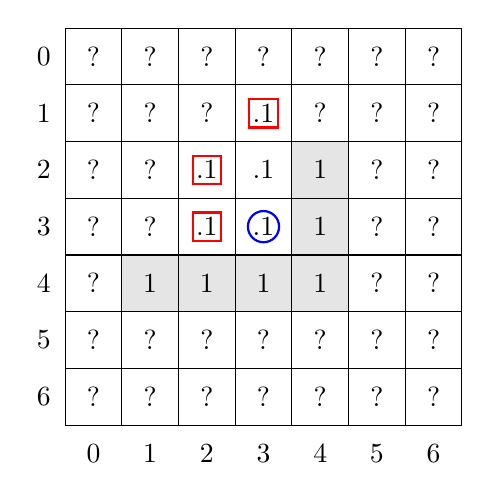
\begin{tikzpicture}[scale=.9]
% Obstacles
\foreach \r/\c in {32/32, 32/24, 32/16, 8/16, 16/16, 24/16}
  \fill[gray!20] (\r mm,\c mm) rectangle +(8mm,8mm);
% Robot
%\fill[gray!50] (24mm,24mm) rectangle +(8mm,8mm);
\draw[blue,thick] (28mm,28mm) circle [radius=2.2mm];
% Frontier
\foreach \r/\c in {18/26, 18/34, 26/42}
  \draw[red,thick] (\r mm,\c mm) rectangle +(4mm,4mm);
% Grid
\draw[step=8mm] (0,0) grid (56mm,56mm);
\foreach \r in {0,1,2,3,4,5,6} {
  \node at (\r*8mm+4mm,-4mm) {\p{\r}};
}
\foreach \r in {0,1,2,3,4,5,6} {
  \node at (-3mm,52mm-\r*8mm) {\p{\r}};
}
% Cells
\foreach \r in {0,1,2,3,4,5,6} {
  \node at (\r*8mm+4mm,52mm) {\p{?}};
}
\foreach \r/\a in {0/?,1/?,2/?,3/.1,4/?,5/?,6/?} {
  \node at (\r*8mm+4mm,44mm) {\p{\a}};
}
\foreach \r/\a in {0/?,1/?,2/.1,3/.1,4/1,5/?,6/?} {
  \node at (\r*8mm+4mm,36mm) {\p{\a}};
}
\foreach \r/\a in {0/?,1/?,2/.1,3/.1,4/1,5/?,6/?} {
  \node at (\r*8mm+4mm,28mm) {\p{\a}};
}
\foreach \r/\a in {0/?,1/1,2/1,3/1,4/1,5/?,6/?} {
  \node at (\r*8mm+4mm,20mm) {\p{\a}};
}
\foreach \r in {0,1,2,3,4,5,6} {
  \node at (\r*8mm+4mm,12mm) {\p{?}};
}
\foreach \r in {0,1,2,3,4,5,6} {
  \node at (\r*8mm+4mm,4mm) {\p{?}};
}
\end{tikzpicture}
\caption{Exploração de um labirinto}\label{fig.map-seven}
\end{center}
\end{figure}

Em Algorithm~\ref{alg.frontier}, o robô usa a distância até uma célula fronteiriça como critério para decidir para onde se mover. Na Fig.~\ref{fig.map-seven} a célula à esquerda do robô a $(3,2)$ é a célula mais próxima, pois está a apenas um passo de distância, enquanto as outras duas células de fronteira estão a dois passos de distância. Podemos considerar um critério diferente, levando em conta o número de células desconhecidas adjacentes a uma célula de fronteira. Começando com uma célula de fronteira com mais células desconhecidas pode tornar o algoritmo mais eficiente. Definimos a prioridade de uma célula de fronteira como:
\[
p_\sub{cell} = \frac{a_\sub{cell}}{d_\sub{cell}}\,,
\]
onde $a_sub{cell}$ é o número de células desconhecidas adjacentes e $d_sub{cell}$ é a distância do robô. As prioridades das três células fronteiriças são:
\[
p_{(3,2)} = 1/1 = 1,\;\;p_{(2,2)} = 2/2 = 1,\;\;p_{(1,3)} = 3/2 = 1.5\,.
\]
A prioridade da célula $(1,3)$ é a mais alta e a exploração começa lá.

\begin{framed}
\act{Algoritmo de fronteira}{frontier}
\begin{itemize}
\item Implementar o algoritmo de fronteira. Você precisará incluir um algoritmo para mover-se com precisão de uma célula para outra e um algoritmo para contornar obstáculos.
\item Executar o programa no mapa da grade na Fig.~\ref{fig.map-explore5}. Você obtém o mesmo caminho? Se não, por que não?
\item Executar o programa no mapa da grade na Fig.~\ref{fig.map-explore5}.
\item Modificar Algoritmo~\ref{alg.frontier} para usar a prioridade descrita em Sect.~\ref{s.priority}. O caminho é diferente daquele gerado pelo programa original?
\item Tente implementar o algoritmo de fronteira em seu robô. Qual é o aspecto mais difícil da implementação?
\end{itemize}
\end{framed}

\section{Mapeamento utilizando o conhecimento do meio ambiente}\label{s.map-update}

Agora que sabemos como explorar um ambiente, vamos considerar como construir um mapa durante a exploração. No Cap.~\ref{ch.local} vimos que um robô pode se localizar com a ajuda de pontos de referência externos e sua representação em um mapa. Sem tais pontos de referência externos, o robô só pode confiar na odometria ou medição inercial, que estão sujeitos a erros que aumentam com o tempo (Fig.~\ref{fig.odo-errors}). Como é possível fazer um mapa quando a localização está sujeita a grandes erros?

Mesmo com má odometria, o robô pode construir um mapa melhor se ele tiver alguma informação sobre a estrutura do ambiente. Suponha que o robô tente construir a planta de uma sala, seguindo suas paredes. Diferenças nas velocidades reais das rodas esquerda e direita levarão o robô a concluir que as paredes não são retas (Fig.~\ref{fig.map-room1}), mas se o robô souber que as paredes são retas e perpendiculares umas \emph{às outras}, o robô pode construir o mapa mostrado na Fig.~\ref{fig.map-room2}. Quando ele encontra uma curva acentuada, ele entende que a curva é um canto de $90^\circ$ onde duas paredes se encontram, portanto seu mapeamento dos ângulos estará correto. Haverá também um erro ao medir o comprimento das paredes e isto pode levar ao intervalo mostrado na figura entre a primeira e a última parede. A figura mostra uma pequena lacuna que não seria importante, mas se o robô estiver mapeando uma grande área, o problema de \emph{fechar um laço} em um mapa é difícil de resolver porque o robô tem apenas uma visão local do ambiente.

\begin{figure}
\begin{minipage}{.45\textwidth}
\begin{tikzpicture}[scale=1.2]
\pic[rotate=90,scale=.5] at (0,0) { robot };
\draw[bend right=10] (-6mm,0mm) to (-10mm,25mm);
\draw[bend right=10] (-10mm,25mm) to (10mm,35mm);
\draw[bend right=10] (10mm,35mm) to (25mm,20mm);
\draw[bend right=10] (25mm,20mm) to (20mm,5mm);
\end{tikzpicture}
\caption{Movimento percebido de um robô baseado na odometria}
\label{fig.map-room1}
\end{minipage}
\hspace{\fill}
\begin{minipage}{.45\textwidth}
\begin{tikzpicture}[scale=1.2]
\pic[rotate=90,scale=.5] at (0,0) { robot };
\draw (-6mm,2mm)  to (-6mm,25mm);
\node at (-8mm,0mm) {\p{lacuna}};
\draw (-6mm,25mm) to (20mm,25mm);
\draw (20mm,25mm) to (20mm,-4mm);
\draw (20mm,-4mm) to (-6mm,-4mm);
\draw (-6mm,-4mm) to (-6mm,-2mm);
\end{tikzpicture}
\caption{Odometria junto com o conhecimento da geometria das paredes}
\label{fig.map-room2}
\end{minipage}
\end{figure}

%\begin{figure}
%\subfigures
%\begin{minipage}{\textwidth}
%\leftfigure{
%\begin{tikzpicture}[scale=1.2]
%\pic[rotate=90,scale=.5] at (0,0) { robot };
%\draw[bend right=10] (-6mm,0mm) to (-10mm,25mm);
%\draw[bend right=10] (-10mm,25mm) to (10mm,35mm);
%\draw[bend right=10] (10mm,35mm) to (25mm,20mm);
%\draw[bend right=10] (25mm,20mm) to (20mm,5mm);
%\end{tikzpicture}
%}
%\hspace{\fill}
%\rightfigure{
%\begin{tikzpicture}[scale=1.2]
%\pic[rotate=90,scale=.5] at (0,0) { robot };
%\draw (-6mm,2mm)  to (-6mm,25mm);
%\node at (-8mm,0mm) {\p{gap}};
%\draw (-6mm,25mm) to (20mm,25mm);
%\draw (20mm,25mm) to (20mm,-4mm);
%\draw (20mm,-4mm) to (-6mm,-4mm);
%\draw (-6mm,-4mm) to (-6mm,-2mm);
%\end{tikzpicture}
%}
%\leftcaption{Perceived motion of a robot based on odometry }\label{fig.map-room1}
%\rightcaption{Odometry together with knowledge of the geometry of the walls}\label{fig.map-room2}
%\end{minipage}
%\end{figure}

Considere um cortador de grama robótico, dada a tarefa de cortar um gramado andando para frente e para trás; ele tem que fechar o laço voltando para sua estação de carga (Fig.~\ref{fig.lawn}). Não é possível implementar este comportamento usando apenas a odometria, uma vez que pequenos erros de velocidade e direção levam a grandes erros na posição do robô. É altamente improvável que através da odometria apenas o robô corte toda a superfície do gramado e retorne a sua estação de carga. Pontos de referência como cabos de sinalização no solo precisam ser usados para fechar o laço.

\begin{figure}
\begin{center}
% Robotic lawnmower
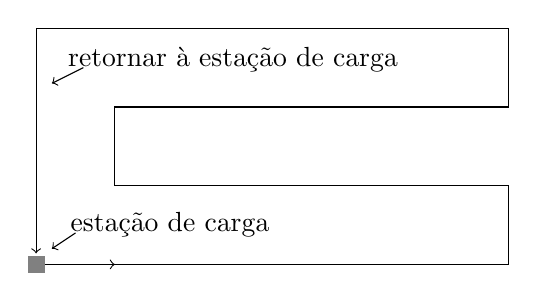
\begin{tikzpicture}[align=left]
\node at (2.5,2.6) {\p{retornar à estação de carga}};
\draw[->] (.6,2.5) -- +(-4mm,-2mm);
\draw (0,0) -- (6,0) -- (6,1) -- (1,1) -- (1,2) -- (6,2) -- (6,3) -- (0,3);
\draw[->] (0,0) -- (1,0);
\draw[->] (0,3) -- (0,4pt);
\draw[fill,gray] (-1mm,-1mm) rectangle +(2mm,2mm);
\node at (1.7,.5) {\p{estação de carga}};
\draw[->] (.5,.4) -- +(-3mm,-2mm);
\end{tikzpicture}
\end{center}
\caption{Um cortador de grama robótico cortando uma área e retornando à sua estação de carga}\label{fig.lawn}
\end{figure}

A construção de mapas pode ser significativamente melhorada usando dados de sensores que podem dar informações sobre características regulares no ambiente, em particular, a uma longa distância. As características regulares podem ser linhas no chão, uma orientação global ou a detecção de características que se \emph{sobrepõem} a outras medidas. Suponha que tenhamos um sensor de distância que possa medir distâncias sobre uma grande área (Fig.~\ref{fig.map_overlap}). A medição sobre uma grande área permite ao robô identificar características tais como paredes e cantos a partir de uma medição feita em um único local. As medições sobre uma grande área facilitam a identificação de sobreposições entre os mapas locais que são construídos em cada local à medida que o robô se move através do ambiente. Comparando os mapas locais, a localização pode ser corrigida e o mapa pode ser atualizado com precisão. Este é o tópico do algoritmo SLAM descrito na próxima seção.

\begin{figure}
\begin{center}
\begin{tikzpicture}[scale=1.2]
\pic[rotate=90,scale=.5] at (0,0) { robot };
\pic[rotate=90,scale=.5] at (0,19mm) { robot };
\pic[scale=.5] at (10mm,28mm) { robot };
\draw[thick,dashed,color=red] (0,2mm) circle[radius=14mm];
\draw[thick,dashed,color=blue] (0,21mm) circle[radius=14mm];
\draw[thick,dashed,color=green!70!black] (12mm,28mm) circle[radius=14mm];
\draw[thick,color=red,yshift=-2pt] (-6mm,-10mm) -- (-6mm,15mm);
\draw[thick,color=blue] (-7mm,9mm) -- (-7mm,33mm) -- (8mm,33mm);
\draw[thick,color=green!70!black] (-1mm,34mm) -- (25mm,34mm);
\end{tikzpicture}
\end{center}
\caption{Medidas de sensor de longo alcance podem detectar sobreposições}\label{fig.map_overlap}
\end{figure}

\begin{framed}
\act{Cortador de grama robótico}{lawnmower}
\begin{itemize}
\item Escreva um programa que faz com que um cortador de grama robótico se mova por um caminho usando apenas a odometria (Fig.~\ref{fig.lawn}). Execute o programa várias vezes. O robô volta para a estação de carga? Se não, de que tamanho são os erros? Os erros são consistentes ou mudam de uma corrida para a próxima?
\item Coloque pontos de referência de fita preta ao redor do gramado (Fig.~\ref{fig.lawn-landmarks}). Programe seu robô para reconhecer os pontos de referência e corrigir sua localização. Quão grandes devem ser os pontos de referência para que o robô os detecte de forma confiável?
\end{itemize}
\end{framed}

\begin{figure}
\begin{center}
% Robotic lawnmower with landmarks
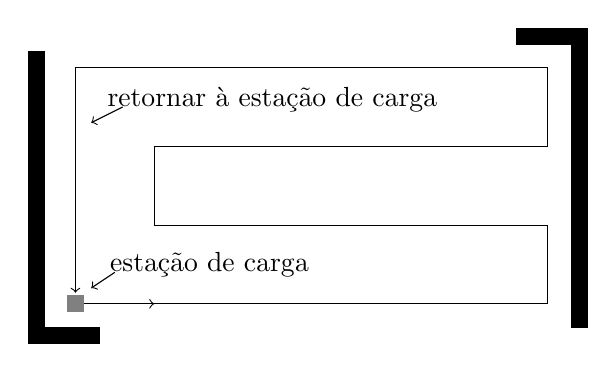
\begin{tikzpicture}[align=left]
\node at (2.5,2.6) {\p{retornar à estação de carga}};
\draw[->] (.6,2.5) -- +(-4mm,-2mm);
\draw (0,0) -- (6,0) -- (6,1) -- (1,1) -- (1,2) -- (6,2) -- (6,3) -- (0,3);
\draw[->] (0,0) -- (1,0);
\draw[->] (0,3) -- (0,4pt);
\draw[fill,gray] (-1mm,-1mm) rectangle +(2mm,2mm);
\node at (1.7,.5) {\p{estação de carga}};
\draw[->] (.5,.4) -- +(-3mm,-2mm);
\draw[fill,black] (-.6,-.4) rectangle +(2mm,3.6);
\draw[fill,black] (-.6,-.5) rectangle +(9mm,2mm);
\draw[fill,black] (6.3,-.3) rectangle +(2mm,3.6);
\draw[fill,black] (6.5,3.3) rectangle +(-9mm,2mm);
\end{tikzpicture}
\end{center}
\caption{Um cortador de grama robótico com pontos de referência}\label{fig.lawn-landmarks}
\end{figure}

\section{Um exemplo numérico para um algoritmo SLAM}\label{s.slam-numerical}

O algoritmo SLAM é bastante complicado, então primeiro calculamos um exemplo numérico e depois damos a apresentação formal.

A figura~\ref{fig.mapping1a} mostra um robô em uma sala em direção ao topo do diagrama. O robô está próximo a um canto da sala e há uma projeção da parede para a esquerda do robô, talvez um pilar de apoio do edifício. Fig.~\ref{fig.mapping1b} é o mapa correspondente. O ponto grande mostra a posição do robô e a seta associada mostra seu cabeçalho. A linha pontilhada grossa representa a parede real. As células brancas representam locais conhecidos por serem livres, as células cinzas representam obstáculos e as células com pontos de interrogação ainda estão inexploradas. Uma célula é considerada como parte do obstáculo se a maioria da área da célula estiver atrás da parede. Por exemplo, os dois segmentos horizontais da projeção da parede estão próximos ao limite das células por onde passam, mas estas células são consideradas parte do obstáculo porque quase toda a sua área está atrás da parede.

\begin{figure}
\begin{minipage}{.45\textwidth}
\includegraphics[width=.4\textwidth]{mappingA.pdf}
\caption{Um robô perto da parede de uma sala}
\label{fig.mapping1a}
\end{minipage}
\hspace{\fill}
\begin{minipage}{.45\textwidth}
\includegraphics[width=.4\textwidth]{mappingB.pdf}
\caption{O mapa correspondente}
\label{fig.mapping1b}
\end{minipage}
\end{figure}

%
%\begin{figure}
%\subfigures
%\begin{minipage}{\textwidth}
%\leftfigure{
%\includegraphics[width=.4\textwidth]{mappingA.pdf}
%}
%\hspace{\fill}
%\rightfigure{
%\includegraphics[width=.4\textwidth]{mappingB.pdf}
%}
%\leftcaption{A robot near the wall of a room}\label{fig.mapping1a}
%\rightcaption{The corresponding map}\label{fig.mapping1b}
%\end{minipage}
%\end{figure}

Com o objetivo de apresentar os detalhes do algoritmo SLAM, o mapa é altamente simplificado. Primeiro, as células são muito grandes demais, aproximadamente do mesmo tamanho do próprio robô. Na prática, as células seriam muito menores do que o robô. Segundo, especificamos que cada célula (explorada) ou é livre (branca) ou contém um obstáculo (cinza); os verdadeiros algoritmos SLAM usam uma representação probabilística (Sect.~\ref{s.grids}).

Suponha que o robô na Fig.~\ref{fig.mapping1a} pretende avançar para a nova posição mostrada na Fig.~\ref{fig.mapping2a}. A Figura~\ref{fig.mapping2b} mostra o mapa correspondente à posição após o movimento pretendido, onde o robô moveu a altura de uma célula para cima a partir de sua posição inicial. Infelizmente, a roda direita se move sobre uma área de baixo atrito e, embora o robô acabe na posição correta, seu rumo está muito distante para a direita. A posição real do robô é mostrada na Fig.~\ref{fig.mapping2c} e a Fig.~\ref{fig.mapping2d} é o mapa correspondente.

\begin{figure}
\begin{minipage}{.45\textwidth}
\includegraphics[width=.43\textwidth]{mapping2A.pdf}
\caption{O movimento pretendido do robô}
\label{fig.mapping2a}
\end{minipage}
\hspace{\fill}
\begin{minipage}{.45\textwidth}
\includegraphics[width=.43\textwidth]{mapping2B.pdf}
\caption{O mapa para o movimento pretendido}
\label{fig.mapping2b}
\end{minipage}
\end{figure}

\begin{figure}
\begin{minipage}{.45\textwidth}
\includegraphics[width=.43\textwidth]{mapping2C.pdf}
\caption{O movimento real do robô}
\label{fig.mapping2c}
\end{minipage}
\hspace{\fill}
\begin{minipage}{.45\textwidth}
\includegraphics[width=.43\textwidth]{mapping2D.pdf}
\caption{O mapa para o movimento real}
\label{fig.mapping2d}
\end{minipage}
\end{figure}
%
%\begin{figure}
%\subfigures
%\begin{minipage}{\textwidth}
%\leftfigure{
%\includegraphics[width=.43\textwidth]{mapping2A.pdf}
%}
%\hspace{\fill}
%\rightfigure{
%\includegraphics[width=.43\textwidth]{mapping2B.pdf}
%}
%\leftcaption{The intended motion of the robot}\label{fig.mapping2a}
%\rightcaption{The map for the intended motion}\label{fig.mapping2b}
%\end{minipage}
%\end{figure}
%
%\begin{figure}
%\subfigures
%\begin{minipage}{\textwidth}
%\leftfigure{
%\includegraphics[width=.43\textwidth]{mapping2C.pdf}
%}
%\hspace{\fill}
%\rightfigure{
%\includegraphics[width=.43\textwidth]{mapping2D.pdf}
%}
%\leftcaption{The actual motion of the robot}\label{fig.mapping2c}
%\rightcaption{The map for the actual motion}\label{fig.mapping2d}
%\end{minipage}
%\end{figure}
%
A Figura~\ref{fig.mapping3a} (que é a mesma da Fig.~\ref{fig.mapping2b}) mostra a percepção do robô porque o robô moveu uma célula para cima em relação ao mapa na Fig.~\ref{fig.mapping1b}. A partir desta posição ele pode detectar o obstáculo à sua esquerda e investigar as células desconhecidas à sua frente.

Entretanto, devido ao erro na odometria, a percepção \emph{real} do robô é diferente. A figura~\ref{fig.mapping3b} mostra a posição real da parede como vista pelo robô sobreposto no topo das células, onde as células são de cor cinza se a maioria de sua área for conhecida por estar atrás da parede. (Examine várias células para verificar se isto é verdade.) Assumimos que o robô pode sentir paredes a uma distância de até cinco vezes o tamanho de uma célula, como mostrado pelo círculo tracejado e também assumimos que o robô sabe que qualquer parede é uma célula de espessura.

\begin{figure}
\begin{minipage}{.45\textwidth}
\includegraphics[width=.43\textwidth]{mapping3A.pdf}
\caption{A percepção pretendida do robô}
\label{fig.mapping3a}
\end{minipage}
\hspace{\fill}
\begin{minipage}{.45\textwidth}
\includegraphics[width=.43\textwidth]{mapping3B.pdf}
\caption{A percepção real do robô}
\label{fig.mapping3b}
\end{minipage}
\end{figure}

%\begin{figure}
%\subfigures
%\begin{minipage}{\textwidth}
%\leftfigure{
%\includegraphics[width=.43\textwidth]{mapping3A.pdf}
%}
%\hspace{\fill}
%\rightfigure{
%\includegraphics[width=.43\textwidth]{mapping3B.pdf}
%}
%\leftcaption{The intended perception of the robot}\label{fig.mapping3a}
%\rightcaption{The actual perception of the robot}\label{fig.mapping3b}
%\end{minipage}
%\end{figure}

Há um claro descasamento entre o mapa atual e os dados do sensor, que deve corresponder à parte conhecida do mapa. Obviamente, o robô não está onde se espera que esteja baseado na odometria. Como este descasamento pode ser corrigido? Assumimos que a odometria dá uma estimativa razoável da posição (posição e direção) do robô. Para cada erro relativamente pequeno possível na postura, calculamos qual seria a percepção do mapa atual e o comparamos com a percepção real computada a partir dos dados do sensor. A posição que dá a melhor combinação é escolhida como a posição real do robô e o mapa atual é atualizado de acordo.

No exemplo, suponha que o robô esteja na célula esperada ou em um de seus quatro vizinhos (esquerda, direita, cima, baixo) e que o cabeçalho do robô esteja correto ou ligeiramente virado para a direita ($15^\circ$ no sentido horário (CW)) ou ligeiramente para a esquerda ($15^\circ$ no sentido anti-horário (CCW)). Os $5\times 3=15$ possíveis poses são mostrados na Fig.~\ref{fig.pos-explore} e a Fig.~\ref{fig.mapping4} mostra a percepção do mapa computado a partir do mapa atual para cada poses. (Para economizar espaço, apenas um fragmento de $8,00\times 5$ do mapa de $12,00\times 8$ é exibido).

\begin{figure}
\begin{center}
\includegraphics[width=0.5\textwidth]{pos-explore.pdf}
\end{center}
\caption{Posições possíveis do robô}\label{fig.pos-explore}
\end{figure}

\begin{figure}
\begin{center}
\includegraphics[width=0.9\textwidth]{mapping4b.pdf}
\end{center}
\caption{Estimativas de percepção do robô para diferentes poses}\label{fig.mapping4}
\end{figure}

O próximo passo é escolher o mapa que melhor se adapta às medidas do sensor. Primeiro, transforme os mapas de $8\times 5$ em matrizes de $8\ vezes 5$, atribuindo $-1$ a células vazias, $+1$ a células de obstáculos e $0$ a outras células. A matriz esquerda na Fig.~\ref{fig.mapping5} está associada ao mapa atual e a matriz central na figura está associada ao mapa de percepção correspondente à posição onde o robô está na célula correta, mas o cabeçalho é $15^\circ$ CW (o elemento central da linha superior da Fig.~\ref{fig.mapping4}).

Para comparar os mapas, multiplique os elementos das células correspondentes. Que $m(i,j)$ seja a célula $(i,j)$'th do mapa atual e $p(i,j)$ seja a célula $(i,j)$'th do mapa de percepção obtido a partir dos valores dos sensores. $S(i,j)$, a \emph{similaridade} de $(i,j)$'th cell, é:
\[
S(i,j) = m(i,j)\, p(i,j)\,,
\]
que também pode ser expressa como:
\[
\begin{array}{l@{\hspace{2em}}l}
S(i,j) = 1 & \textrm{if}\;\;m(i,j) \neq 0,\, p(i,j) \neq 0,\, m(i,j) = p(i,j)\\
S(i,j) = -1 & \textrm{if}\;\;m(i,j) \neq 0,\, p(i,j) \neq 0,\,  m(i,j) \neq p(i,j)\\
S(i,j) = 0 & \textrm{if }m(i,j) = 0\, \textrm{or}\; p(i,j) = 0\,.
\end{array}
\]
A matriz direita na Fig.~\ref{fig.mapping5} mostra o resultado deste cálculo para as duas matrizes à sua esquerda. Existem muitos significados de $1$ que as matrizes são semelhantes e, portanto, podemos concluir que os mapas de percepção são semelhantes. Para um resultado quantitativo, calcular a soma das similaridades para obter um valor único para qualquer par $m,p$:
\[
\mathcal{S} = \sum_{i=1}^8 \sum_{j=1}^5 S(i,j)\,.
\]

\begin{figure}
\begin{center}
\includegraphics[width=\textwidth]{mapping5.pdf}
\end{center}
\caption{Computação da correspondência entre dois mapas}\label{fig.mapping5}
\end{figure}

A tabela~\ref{tab.matching} dá os valores da similaridade $\mathcal{S}$ para todos os mapas de percepção na Fig.~\ref{fig.mapping4} em comparação com o mapa atual. Como esperado, a maior similaridade é obtida para o mapa correspondente à pose com a posição correta e com o cabeçalho girado por $15^\circ$ CW.

\begin{table}
\caption{Similaridade $\mathcal{S}$ do mapa baseado em sensores com o mapa atual}
\label{tab.matching}
\renewcommand{\arraystretch}{1.2}
\setlength{\tabcolsep}{8pt}
\begin{tabular}{p{22mm}ccc}
\hline\noalign{\smallskip}
&Orientação pretendida&$15^{\circ}$ CW&$15^{\circ}$ CCW\\
Posição pretendida & $22$ & \boldmath $32$ & $20$\\
Subir uma célula       & $23$ & $25$ & $16$\\
Abaixo de uma célula     & $19$ & $28$ & $21$\\
Deixou uma célula     & $6$  & $7$  & $18$\\
Uma célula à direita    & $22$ & $18$ & $18$\\
\noalign{\smallskip}\hline\noalign{\smallskip}
\end{tabular}
\end{table}

Uma vez obtido este resultado, corrigimos a pose do robô e usamos os dados do mapa de percepção para atualizar o mapa atual armazenado na memória do robô. (Fig.~\ref{fig.final-map}).

\begin{figure}
\begin{center}
\includegraphics[width=\textwidth]{final-map.pdf}
\end{center}
\caption{Mapa antes e depois da atualização utilizando dados do mapa de percepção}\label{fig.final-map}
\end{figure}
\smallskip

\section{Atividades para demonstrar o algoritmo SLAM}\label{s.slam-activities}

As duas atividades a seguir demonstram aspectos do algoritmo SLAM. A atividade~\ref{act.computed-perceptions} segue o algoritmo e é destinada à implementação em software. A atividade~\ref{act.measured-perceptions} demonstra um elemento chave do algoritmo que pode ser implementado em um robô educacional.

As atividades são baseadas na configuração mostrada na Fig.~\ref{fig.slam-config}. O robô está localizado na origem do sistema de coordenadas com a pose $((x,y),\theta)=((0,0),0^\circ)$. \footnote{é conveniente tomar o título do robô como $0^\circ$.} Dada a incerteza da odometria, o robô pode estar localizado em qualquer uma das coordenadas $(-1,0), (1,0), (0,-1), (0,1), (0,1)$ e sua orientação pode ser qualquer uma das coordenadas $-15^\circ{}, 0, -15^\circ$ (como mostrado pelas setas tracejadas), dando $15$ de poses possíveis. Os três pontos cinzas nas coordenadas $(2,2), (2,0), (2,-2)$ representam obstáculos conhecidos no mapa atual. (Para economizar espaço, os pontos são exibidos nas coordenadas $(2,1), (2,0), (2,-1)$.) Os obstáculos podem ser detectados por vários sensores de proximidade horizontais, mas para os propósitos das atividades especificamos que existem três sensores.

\begin{figure}
\begin{center}
% SLAM algorithm
\begin{tikzpicture}
\draw[step=3cm,very thin,gray] (-3.01,-3.01) grid (6,3);
% The obstacles
\fill[gray!80!black] (6,0) circle[radius=6pt];
\fill[gray!80!black] (6,3) circle[radius=6pt];
\fill[gray!80!black] (6,-3) circle[radius=6pt];
% The robots
\pic at (0,0) { robot };
\pic at (3,0) { robot };
\pic at (-3,0) { robot };
\pic at (0,3) { robot };
\pic at (0,-3) { robot };
% The three arrows on each robot
\foreach \x/\y in {0/0, 3/0, -3/0, 0/3, 0/-3} {
  \draw[dashed,->,thick] (\x,\y) -- +( 20:15mm);
  \draw[dashed,->,thick] (\x,\y) -- +(  0:15mm);
  \draw[dashed,->,thick] (\x,\y) -- +(-20:15mm);
}
\node at (-3.6,-2.9) {$(-1,-1)$};
\node at (3,3.3) {$(1,1)$};
\end{tikzpicture}
\caption{Configuração para o algoritmo SLAM}\label{fig.slam-config}
\end{center}
\end{figure}

No algoritmo SLAM, o \emph{percepção} de um obstáculo é o valor retornado por um sensor de distância. Para evitar ter que definir modelo para os sensores, as atividades definirão uma percepção como a \emph{distance} e a \emph{head} do sensor para o obstáculo.

\begin{framed}
\act{Localizar o robô a partir das percepções computadas}{computed-perceptions}
\begin{itemize}
\item Para cada uma das poses de $15$, computar o conjunto de percepções de cada obstáculo. Por exemplo, se o robô estiver na pose $((0,0,1,0),-15,0^\circ)$, o conjunto de percepções dos três obstáculos é:
\[
[( 2.2,  41.6^\circ),\,  ( 2.2, -11.6^\circ),\,  ( 3.6, -41.3^\circ)]\,.
\]
\item Dado um conjunto de percepções medidas, calcule suas semelhanças com as percepções das poses de $15$ do robô. Escolha a pose com a melhor semelhança como a pose real do robô. Por exemplo, para o conjunto de percepções medidas:
\[
[( 2.0,  32.0^\circ),\,  ( 2.6, -20.0^\circ),\,  ( 3.0, -30.0^\circ)]\,,
\]
e a similaridade calculada como a soma das diferenças absolutas dos elementos das percepções, a pose com a melhor semelhança é $((0.0, 1.0),-15.0^\circ)$.
\item Experiência com diferentes funções de similaridade.
\item Calculamos que a pose do robô é aproximadamente $((0,0, 1,0),-15,0^\circ)$. Suponha que um novo obstáculo seja colocado na coordenada $(3,0)$. Calcule a percepção de $(d,\theta)$ do objeto desta pose e depois calcule a coordenada $(x,y)$ do novo obstáculo. O novo obstáculo pode ser adicionado ao mapa com esta coordenada.
\item A coordenada computada é significativamente diferente da coordenada $(3,0)$ que seria obtida se o robô estivesse na posição pretendida. $((0,0),0^\circ)$?
\end{itemize}
\end{framed}

\begin{framed}
\act{Localizar o robô a partir das percepções medidas}{measured-perceptions}
\begin{itemize}
\item Coloque três objetos como mostrado na Fig.~\ref{fig.slam-config}.
\item Escrever um programa que armazena o conjunto de valores retornados pelos três sensores de proximidade horizontais. Coloque seu robô sucessivamente em cada uma das poses de $15$ e registre os conjuntos de valores. Agora você tem um banco de dados de percepções: um conjunto de três leituras de sensores para cada posiçao.
\item Colocar o robô em uma das poses e armazenar o conjunto de valores retornados pelos sensores. Calcule a similaridade deste conjunto com cada um dos conjuntos no banco de dados. Exibir a pose associada com a melhor semelhança.
\item Experimentar a colocação do robô em várias poses e várias vezes em cada pose. Quão precisa é a determinação da pose?
\item Experimentar com diferentes funções de similaridade.
\end{itemize}
\end{framed}

\section{A formalização do algoritmo SLAM}\label{s.slam-formal}

Algoritmo~\ref{alg.slam} é um algoritmo SLAM que encontra a posição cujo mapa de percepção é o mais próximo do mapa de percepção obtido a partir dos dados do sensor. O robô é localizado a esta posição e o mapa é atualizado para o que é percebido nesta posição.

\begin{figure}
\begin{alg}{SLAM}{slam}
\hline
&\idv{}matrix $\vec{m}$ \ass partial map&// Current map\\
&\idv{}matrix $\vec{p}$&// Perception map\\
&\idv{}matrix $\vec{e}$&// Expected map\\
&\idv{}coordinate $\vec{c}$ \ass initial position&// Current position\\
&\idv{}coordinate $\vec{n}$&// New position\\
&\idv{}coordinate array $\vec{T}$&// Set of test positions\\
&\idv{}coordinate $\vec{t}$&// Test position\\
&\idv{}coordinate $\vec{b}$ \ass none&// Best position\\
\hline
\stl{}&loop&\\
\stl{}&\idc{}move a short distance&\\
\stl{}&\idc{}$\vec{n}$ \ass odometry($\vec{c}$)&// New position based on odometry\\
\stl{}&\idc{}$\vec{p}$ \ass analyze sensor data&\\
&&\\
\stl{}&\idc{}for every $\vec{t}$ in $\vec{T}$&// T is the positions around n\\
\stl{}&\idc{}\idc{}$\vec{e}$ \ass expected($\vec{m}$, $\vec{t}$)&// Expected map at test position\\
\stl{}&\idc{}\idc{}if compare($\vec{t}$,$\vec{e}$) better than $\vec{b}$&\\
\stl{}&\idc{}\idc{}\idc{}$\vec{b}$ \ass $\vec{t}$&// Best test position so far\\
&&\\
\stl{}&\idc{}$\vec{n}$ \ass $\vec{b}$&// Replace new position by best position\\
\stl{}&\idc{}$\vec{m}$ \ass update($\vec{m}$,$\vec{p}$,$\vec{n})$&// Update map based on new position\\
\stl{}&\idc{}$\vec{c}$ \ass $\vec{n}$&// Current position is new position\\
\end{alg}
\end{figure}

O algoritmo é dividido em três fases. Na primeira fase (linhas~2--4), o robô se move a uma curta distância e sua nova posição é computada por odometria. O mapa de percepção neste local é obtido através da análise dos dados do sensor.

Assumindo que o erro de odometria é relativamente pequeno, podemos definir um conjunto de posições de teste onde o robô pode estar. Na segunda fase (linhas~5--8), o mapa esperado em cada uma destas posições é computado e comparado com o mapa atual. A melhor correspondência é salva.

Na terceira fase (linhas~9--11), a posição com a melhor correspondência torna-se a nova posição e o mapa atual é atualizado de acordo.

Na prática, o algoritmo é um pouco mais complicado porque tem que levar em conta que o mapa de percepção obtido a partir dos sensores é limitado pelo alcance dos sensores. A sobreposição será parcial tanto porque o alcance dos sensores não cobre todo o mapa atual quanto porque os sensores podem detectar obstáculos e áreas livres fora do mapa atual. Portanto, o tamanho do mapa de percepção $\vec{p}$ será muito menor do que o mapa esperado $\vec{e}$ e a função \p{compare(}$\vec{p}$\p{,}$\vec{e}$\p{)} somente comparará as áreas que se sobrepõem. Além disso, ao atualizar o mapa atual, serão adicionadas áreas que não estavam anteriormente no mapa. Na Fig.~\ref{fig.final-map} há células no mapa atual que estão fora do raio de cinco células do sensor e não serão atualizadas. As células vermelhas claras eram desconhecidas no mapa atual como indicado pelos pontos de interrogação, mas no mapa de percepção elas agora são conhecidas como parte do obstáculo. Esta informação é usada para atualizar o mapa atual para obter um novo mapa atual.

\section{Sumário}

O movimento robótico preciso em um ambiente incerto exige que o robô tenha um mapa do ambiente. O mapa deve ser mantido no computador do robô; pode ser um mapa em grade de células ou uma representação gráfica de um mapa contínuo. Em um ambiente incerto, um mapa normalmente não estará disponível para o robô antes de ele iniciar suas tarefas. O algoritmo de fronteira é usado por um robô para construir um mapa enquanto ele explora seu entorno. Mapas mais precisos podem ser construídos se o robô tiver algum conhecimento de seu ambiente, por exemplo, que o ambiente é o interior de um edifício composto de salas e corredores retangulares. Os algoritmos de localização e mapeamento simultâneo (SLAM) usam um processo iterativo para construir um mapa, ao mesmo tempo em que corrigem os erros de localização.

\section{Leitura adicional}

Dois livros didáticos sobre planejamento de caminhos e movimentos são \cite{latombe,lavalle}. Ver também \cite[Capítulo 6]{siegwart}.

O algoritmo de fronteira foi proposto por Yamauchi \cite{yamauchi} que mostrou que um robô poderia usar o algoritmo para explorar com sucesso um escritório com obstáculos.

Algoritmos para SLAM usam probabilidade de uso, em particular a regra Bayes. Os métodos probabilísticos em robótica são o tema do livro didático \cite{thrun}.

Um tutorial em duas partes sobre SLAM de Durrant-Whyte e Bailey pode ser encontrado em \cite{slam-tutorial1,slam-tutorial2}. Um tutorial em duas partes sobre SLAM baseado em gráficos é \cite{slam-graph}.

O curso online de Sebastian Thrun é útil: \par\url{https://classroom.udacity.com/courses/cs373}.

